\section{Videojuegos educativos}

Los videojuegos educativos o lúdicos son una herramienta que permite a los estudiantes desarrollar competencias en sus procesos de aprendizaje. Esta se encuentra dentro de la clasificación por género de ``otros" que se ha descrito antes. Aquí segun informes del Horizon (New Media Consortium) como Games and gamification \cite{vid07} resaltan la gamificación como una de las principales procesos de aprendizaje con mayor crecimiento, que también se ha descrito con anterioridad. 
\\[1pt]

Su ventaja es que el ser humano aprende jugando por eso es que un videojueggo educativo es una gran ayuda. Desde los primeros años de vida un niño adquiere conocimientos a través del juego. Ya que para la psicóloga infantil, esta característica permite al infante socializar en un entorno completamente nuevo, que lo estimula a conocer muchos aspectos de la realidad. Además de ser emocionante y entretenido, otra ventaja es que le permite al jugador desarrollar un nivel de pensamiento creativo para enfrentar las circunstancias de la vida. A diferencia de un adulto que tiene temor a equivocarse, un niño juega, se equivoca, lo vuelve a intentar, y de esa experiencia aprende. Esta afirmación anterior ahora se puede aplicar a cualquier persona, pues en un videojuego no existe el riesgo de equivocarse.
\\[1pt]

El videojuego se puede utilizar como un instrumento del proceso enseñanza-aprendizaje. Según el Dr. Francisco Revuelta, especialista en procesos de formación en espacios virtuales dentro del ámbito pedagógico, un videojuego educativo es dividido en dos vertientes según su forma de enseñanza-aprendizaje. La primera, como un simulador de aprendizaje o herramienta en el cual se puede comprobar el nivel de competencia del alumno de acuerdo a las exigencias que le propone el videojuego, como ejemplo la imagen \ref{fig:mine} muestra el juego Minecraft education edition. La segunda, como un entorno virtual de aprendizaje donde el estudiante es motivado a resolver problemas académicos interactuando dentro del espacio brindado por el videojuego\cite{vid06} como ejemplo la imagen \ref{fig:lea} muestra la Plataforma learny.
\\[1pt]

	\begin{figure}
		\centering
	\caption{Simulador de aprendizaje: Minecraft education edition}
		\label{fig:mine}
		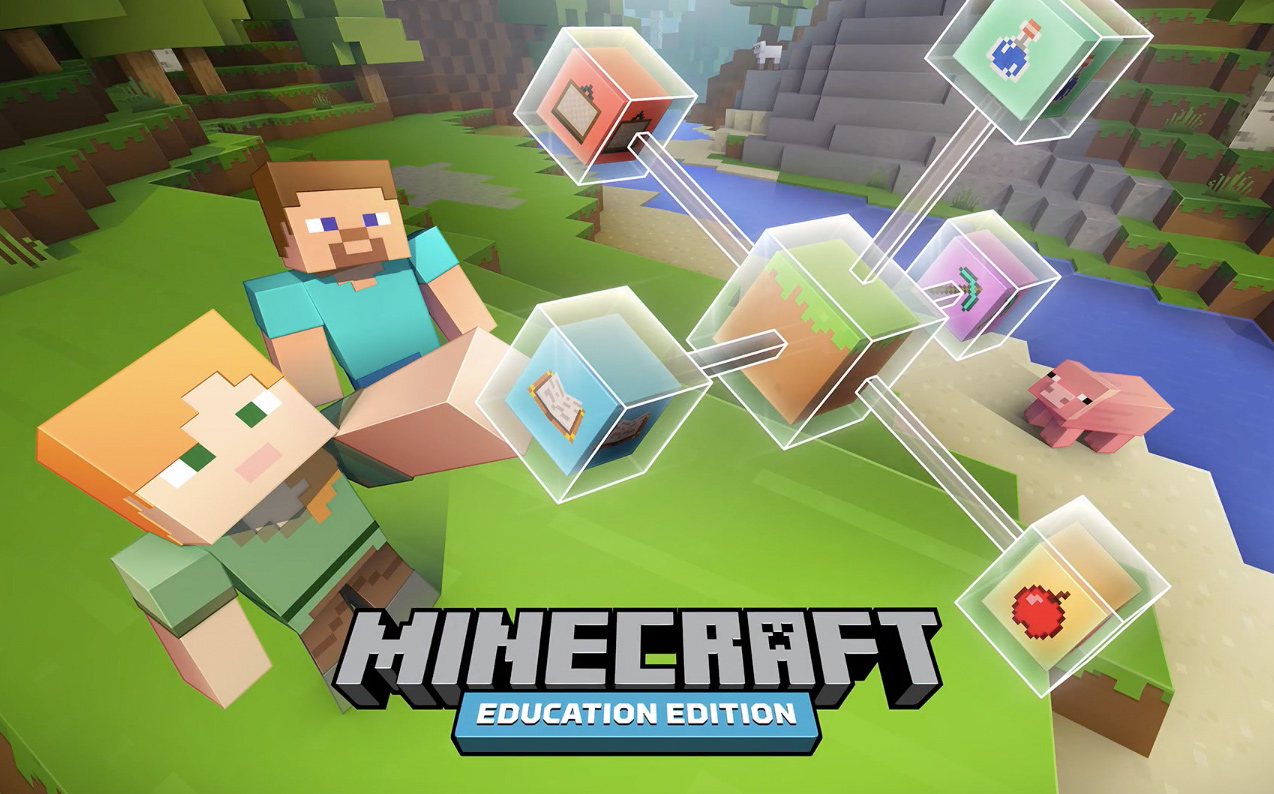
\includegraphics[width=0.5\textwidth]{03MarcoTeorico/imageR/minecraft}
\end{figure}
	\begin{figure}
	\centering
		\caption{Entorno virtual: Plataforma learny}
		\label{fig:lea}
		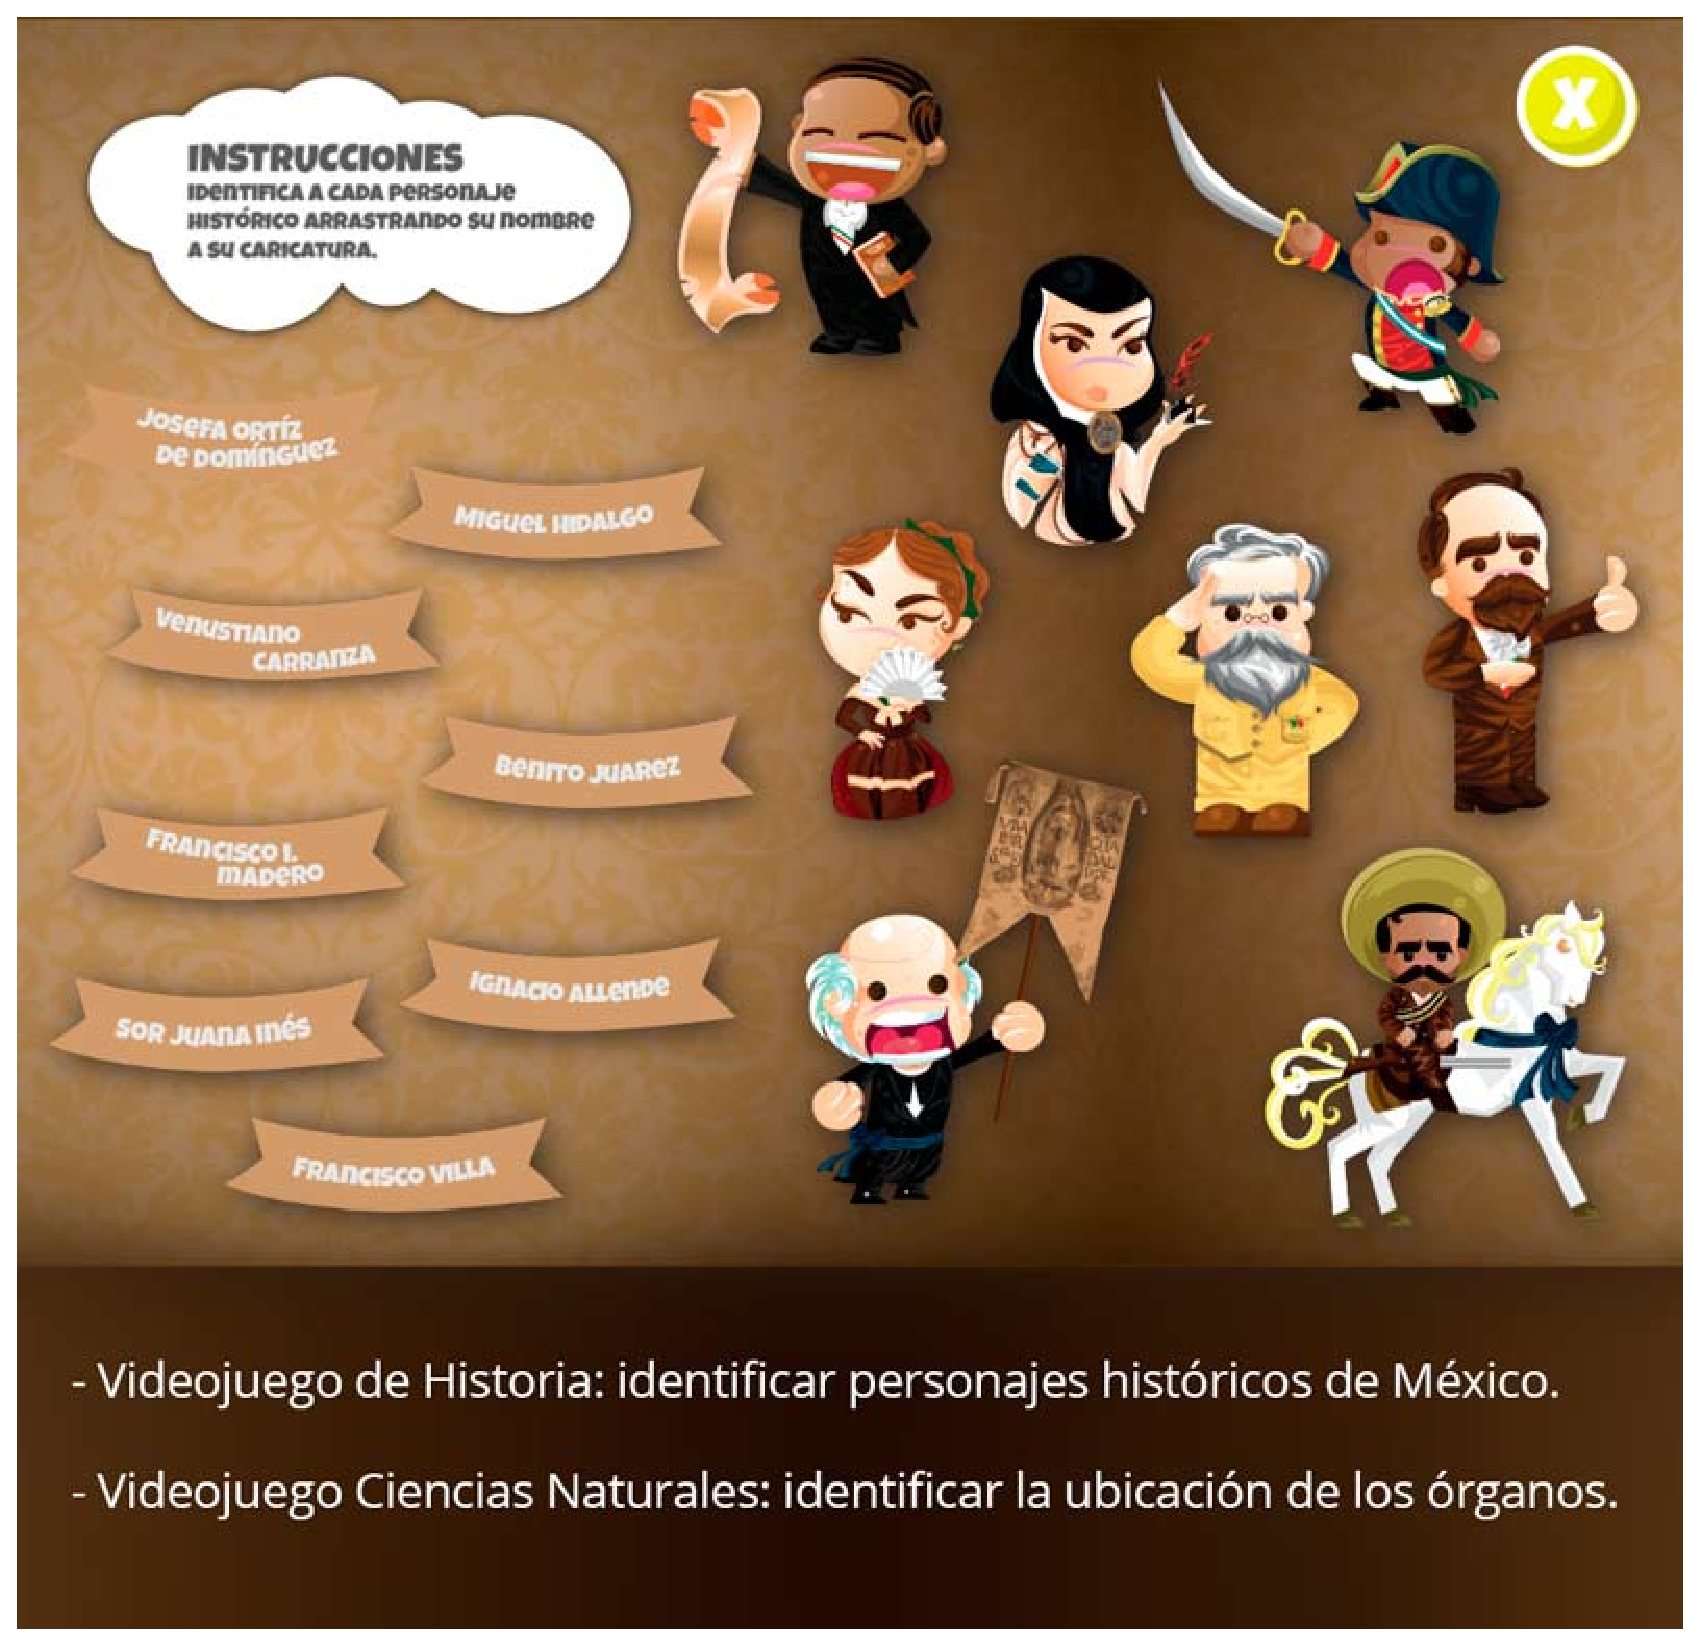
\includegraphics[width=0.5\textwidth]{03MarcoTeorico/imageR/learny}
\end{figure}

Como consecuencia el videojuego aumenta la motivación en el aprendizaje, ayuda al alumno a adquirir conocimientos de una manera atractiva y contribuye al desarrollo de competencias. Pero en contra parte, un videojuego educativo nunca podrá sustituir por completo la enseñanza tradicional como un salón de clases, un videojuego educativo sólo sirve como complemento y herramienta para el proceso de enseñanza-aprendizaje.
\\[1pt]
